\documentclass[letterpaper]{article}
\usepackage{aaai}
\usepackage{times}
\usepackage{helvet}
\usepackage{courier}
\usepackage{graphicx}
\frenchspacing
\setlength{\pdfpagewidth}{8.5in}
\setlength{\pdfpageheight}{11in}
\pdfinfo{
/Title (Insert Your Title Here)
/Author (Put All Your Authors Here, Separated by Commas)}
\setcounter{secnumdepth}{0}  
 \begin{document}
% The file aaai.sty is the style file for AAAI Press 
% proceedings, working notes, and technical reports.
%
\title{Handwritten Font Generator \\ Based on StyleGAN}
\author{Chengruidong Zhang, Haoran Xi}
\maketitle

\section{Problem Statement}
A font consists of a set of character images sharing the same style. Because each character has a fixed skeleton, we may be able to extract the style information from limited character images and apply it to all characters. This means that a new font can be created with very few character images as input, and everyone can create his / her handwritten font without writing all the characters.

\begin{center}
    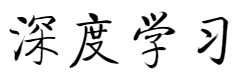
\includegraphics[]{proposal-fig-qiti.png}
    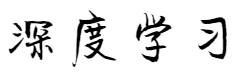
\includegraphics[]{proposal-fig-jinglei.png}

    Figure 1. Same characters in different fonts.\\The second font is more uneven and compact.
\end{center}


\section{Related Works}

\section{Dataset}
The dataset includes $32 \times 32$ images of common characters converted from different font files. System fonts such as Brush Script MT and Segoe Script can be used at the beginning. More handwritten fonts will be collected if necessary. We plan to start with English characters and numbers, and then then introduce Chinese characters.

\section{Model}
We plan to build a Generative Adversarial Network, which consists of a 5-layer Style-based generator and a 3-layer conditional discriminator. The input and output are both $32 \times 32$ single-channel (black and white) images.
\\
On each training epoch, images of two different fonts are fed into the model, providing skeleton and style information, respectively.
\\
Denote an image of character $c$ and font $f$ by $I[c,f]$. For each time, the generator takes a pair of images $(I_1=I[c_i,f_0], I_2=I[c_j,f_k])$ and outputs an image $I_o$ with skeleton of $I_1$ and style of $I_2$. The discriminator differs the output from the groundtruth - image $I[c_i,f_k]$. Font $f_0$ should have clear skeletons, and can the same whenever training or testing.

\section{Anticipated Outcomes}
To be specific, the generator is expected to (1) separate the structure and style information of a image and (2) apply the style information to another image. The discriminator should be able to tell whether a pair of images describe the same character and belong to the same font.
\\
Therefore, a well-trained generator can generate images of any character in the style of any input image $I_2$. If we input a handwritten character image repeatly with all common characters $I[c_i,f_0]$, we'll get a new handwritten font.

\section{Challanges and Concerns}
\begin{itemize}
    \item The typical StyleGAN extracts style information using full-connected networks, which may not be able to seperate the style and skeleton of character pictures well. We may need a pre-trained skeleton extractor rather than roughly putting images into the generator.
    \item The skeleton provider, $I[c_i,f_0]$, also plays the role of identifier. If our generator have the ability to remember the skeleton shape of all characters, we can replace the input $I_1$ of one-hot character codes.
    \item Notice that fonts are stored in the form of vector graphs of quadratic Bezier curves. The final model should include a image trace module to output vector graphs.
\end{itemize}

\section{Reference}

\bibliography{proposal-reference.bib}
\bibliographystyle{aaai}
\end{document}